\documentclass[aspectratio=169,fleqn]{beamer}
\usepackage{spc}
\usepackage{graphicx}
\begin{document}

\begin{frame}
  \title{\vspace{-5ex}\darkblue Scoping the next stock assessment
    platform\\[2ex]
    \it\large\darkgray
    Project 123 progress update and outline of options}
  \author{\vspace{-10ex}\darkgray\bf
    Arni Magnusson, Nick Davies,\\[0.5ex]
    Graham Pilling, Paul Hamer}
  \date{\darkgreen WCPFC Scientific Committee Meeting (SC20)\\[0.5ex]
    Manila, 14 August 2024}
  \titlepage
\end{frame}

% ______________________________________________________________________________

\begin{frame}{Overview}
  \begin{itemize}
    \item[] {\bf\darkblue Introduction} \comment{background, project outline,
      existing software, new development}\\[5ex]
    \item[] {\bf\darkblue Possible Tasks} \comment{migrate assessments to
      existing software, model exploration,\\
      \h{19.5ex}software development}\\[5ex]
    \item[] {\bf\darkblue Timeline} \comment{PAW 2024, expert meeting 2024,
      workshops 2024--2026,\\
      \h{13ex}launching the main project}\\[5ex]
    \item[] {\bf\darkblue Required Resources} \comment{collaboration with other
      tRFMOs,\\
      \h{25.3ex}SPC staff positions \& consultants}\\[1ex]
  \end{itemize}
\end{frame}

% ______________________________________________________________________________

\begin{frame}{The need to to migrate to new software}
  \begin{itemize}
    \item[] MULTIFAN-CL (MFCL) has been used in SPC tuna assessments since
    1990s\\[4ex]
    \item[] MFCL team (Dave Fournier, John Hampton, Nick Davies) retiring in the
    2020s\\[4ex]
    \item[] Development of new features is slowing down\\[4ex]
    \item[] Resources are being allocated to succession plans\\[4ex]
  \end{itemize}
\end{frame}

% ______________________________________________________________________________

\begin{frame}{Project outline}
  This scoping project is scheduled from 1 Feb 2024 to 31 Dec 2026. It
  will:\\[3ex]
  \begin{itemize}
    \item[] Evaluate features and capabilities that will be important in future
    tuna assessments\\[3ex]
    \item[] Explore fitting models to tuna data using existing software
    platforms\\[3ex]
    \item[] Guide decisions on what kind of new software development will be
    required\\[3ex]
    \item[] Establish collaboration with tRFMOs and research labs to achieve these
    goals\\[3ex]
  \end{itemize}
\end{frame}

% ______________________________________________________________________________

\begin{frame}{Stock assessment software}
  Existing software, ready for multi-region tuna assessments\\[3ex]
  \begin{itemize}
    \item[-] {\bf Stock Synthesis} is used by IATTC, IOTC, and ICCAT\\[3ex]
    \item[-] {\bf Gadget} has many features relevant for tuna assessments\\[3ex]
    \item[-] {\bf Casal} has many features relevant for tuna assessments\\[4ex]
  \end{itemize}
  These could be extended further as needs arise\\[2ex]
\end{frame}

% ______________________________________________________________________________

\begin{frame}{Stock assessment software}
  Software that could be developed further:\\[3ex]
  \begin{itemize}
    \item[-] {\bf sbt} is built around CKMR, currently for single-region
    assessments\\[3ex]
    \item[-] {\bf ALSCL} is a state-space model that fits length comps, currently
    no catches\\[3ex]
    \item[-] {\bf WHAM$\,$\raisebox{0.15ex}{+}$\,$Length} is a state-space that fits
    length comps, currently single-region\\[3ex]
    \item[-] {\bf SAM$\,$\raisebox{0.15ex}{+}$\,$Length} is an early exploration
    of extending SAM to fit length comps\\[3ex]
    \item[-] {\bf Stock Synthesis$\,$\raisebox{0.15ex}{+}$\,$Enhanced Tags} is a
    proposed enhancement of the tag module\\[2ex]
  \end{itemize}
\end{frame}

% ______________________________________________________________________________

\begin{frame}{Stock assessment software}
  Also relevant:\\[4ex]
  \begin{itemize}
    \item[-] {\bf Stock Synthesis$\,$\raisebox{0.15ex}{+}$\,$CKMR} is an
    experimental add-on, not included in core software\\[4ex]
    \item[-] {\bf FIMS}, NOAA project coordinating the development of a
    next-generation framework\\[6ex]
  \end{itemize}
\end{frame}

% ______________________________________________________________________________

\begin{frame}{Stock Synthesis}
  Also relevant:\\[4ex]
  \begin{itemize}
    \item[-] {\bf Stock Synthesis$\,$\raisebox{0.15ex}{+}$\,$CKMR} is an
    experimental add-on, not included in core software\\[4ex]
    \item[-] {\bf FIMS}, NOAA project coordinating the development of a
    next-generation framework\\[6ex]
  \end{itemize}
\end{frame}

% ______________________________________________________________________________

\begin{frame}{Possible tasks for SPC to prioritize}
  Subject to SC advice:\\[4ex]
  \begin{enumerate}
    \item Move the {\green swordfish} assessment to Stock Synthesis\\
    \comment{\gray relatively simple compared to other SPC assessments}\\[3ex]
    \item Move the {\green striped marlin} assessment to Stock Synthesis\\
    \comment{\gray also relatively simple}
  \end{enumerate}
\end{frame}

% ______________________________________________________________________________

\begin{frame}{Possible tasks for SPC to prioritize}
  Subject to SC advice and funding approvals by WCPFC:\\[4ex]
  \begin{enumerate}\setcounter{enumi}{2}
  \item Conduct model exploration to fit Casal/Gadget/Stock Synthesis to
  albacore tuna\\
  . The South Pacific albacore assessment model is simpler than the
  other tuna species and therefore a candidate to be the~first tuna stock
  assessment to consider for migration from MFCL. Also, for the next South
  Pacific albacore assesment there may be CKMR information available to
  incorporate in the assessment.
  \item Conduct model exploration to fit Casal/Gadget/Stock Synthesis to the
  original five-region yellowfin tuna dataset. The yellowfin assessment is a
  good candidate to test the capabilities of these software platforms for tuna
  assessments involving multiple regions, tags, and a large number of fisheries.
  The yellowfin tuna assessment is similar to bigeye tuna but runs slightly
  faster, thanks to the simpler \mbox{five-region} structure that was adopted in
  the 2023 assessment.
  \item Conduct model exploration to fit models using a variety of existing
  software to a simplified single-region yellowfin tuna dataset. Models of
  interest include ALSCL, Casal, Gadget, MFCL, sbt, Stock Synthesis, and
  WHAM+Length.
  \end{enumerate}
\end{frame}

% ______________________________________________________________________________

\begin{frame}{Transition plan}
  \vspace{1ex}
  ~\h{-3ex}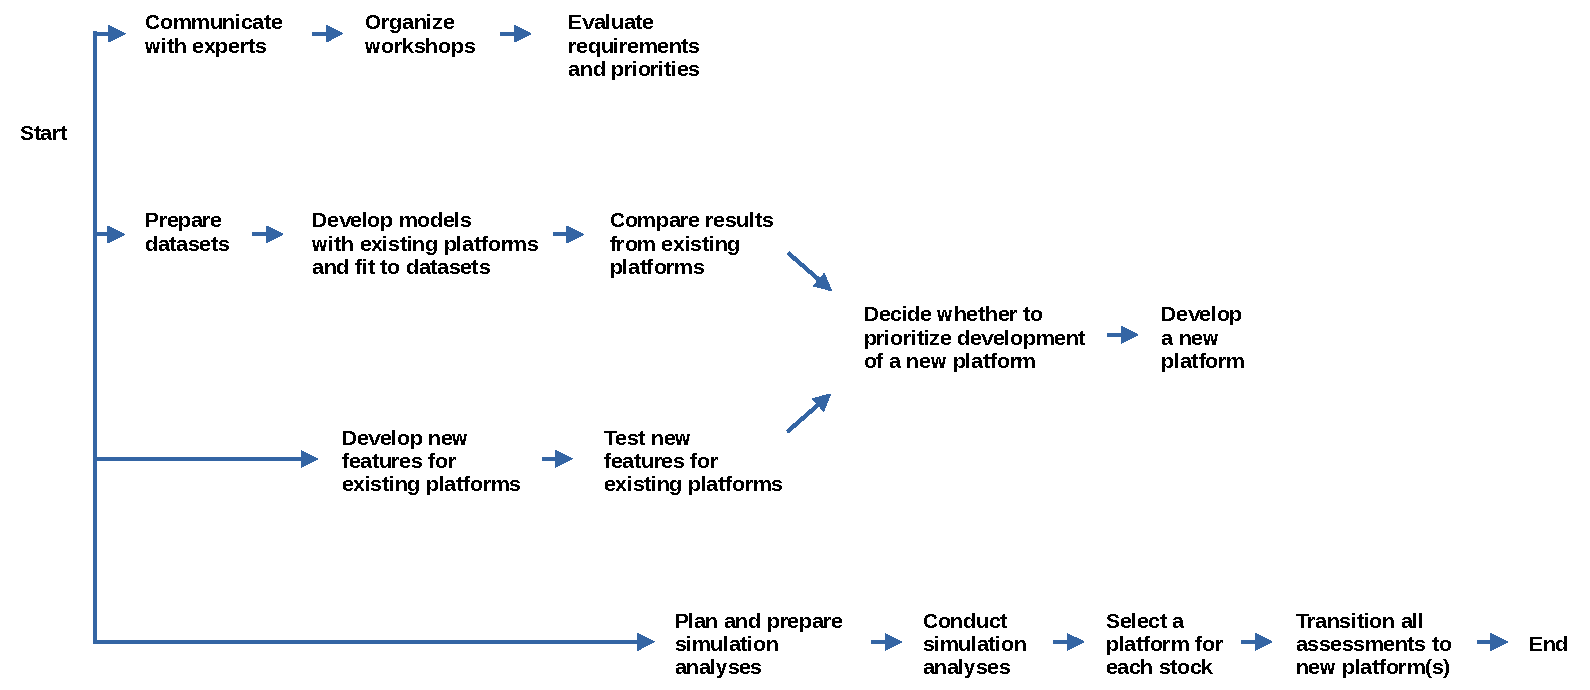
\includegraphics[width=1.05\textwidth]{p123_diagram}
\end{frame}

% ______________________________________________________________________________

\begin{frame}{Summary}
  \begin{itemize}
    \item[] {\bf\darkblue Introduction} \comment{background, project outline,
      existing software, new development}\\[5ex]
    \item[] {\bf\darkblue Possible Tasks} \comment{migrate assessments to
      existing software, model exploration,\\
      \h{19.5ex}software development}\\[5ex]
    \item[] {\bf\darkblue Timeline} \comment{PAW 2024, expert meeting 2024,
      workshops 2024--2026,\\
      \h{13ex}launching the main project}\\[5ex]
    \item[] {\bf\darkblue Required Resources} \comment{collaboration with other
      tRFMOs,\\
      \h{25.3ex}SPC staff positions \& consultants}\\[1ex]
  \end{itemize}
\end{frame}

\end{document}
